\documentclass{beamer}
\usepackage[utf8]{inputenc}
\usepackage[T1]{fontenc}
\usepackage{graphicx}
\usepackage{tikz}

\usecolortheme{beaver}

\title[Voronoi Tessellation]{Voronoi Tessellation: An Overview}
\author{Max Comstock}
\date{March 16, 2018}

\begin{document}

\frame{\titlepage}

\begin{frame}
  \frametitle{Points in space}
  \begin{itemize}
  \item 2-D:\@ identified with $(x, y)$ coordinates
  \item Any dimension (harder to draw): $(x_1, x_2, \ldots, x_n)$
  \item Can define a distance function $d$ between two points (usually Euclidean distance)
  \end{itemize}
  \begin{center}
    \begin{tikzpicture}
      \filldraw (3,1) circle (2pt) node[below] {$(3,1)$};
      \filldraw (-0.5,-2) circle (2pt) node[left] {$(-0.5,-2)$};
      \filldraw (-1,2) circle (2pt) node[below] {$(-1,2)$};
      \filldraw (2,-1) circle (2pt) node[below] {$(2,-1)$};
      \filldraw (-3,-1) circle (2pt) node[below] {$(-3,-1)$};
      \filldraw (0.5,0.5) circle (2pt) node[right] {$(0.5,0.5)$};
      \filldraw (1,2) circle (2pt) node[below] {$(1,2)$};
      \draw[<->] (-4,0) -- (4,0) coordinate (x axis);
      \draw[<->] (0,-2.5) -- (0,2.5) coordinate (y axis);
    \end{tikzpicture}
  \end{center}
\end{frame}

\begin{frame}
  \frametitle{An example Voronoi diagram}
  \begin{center}
    \only<1>{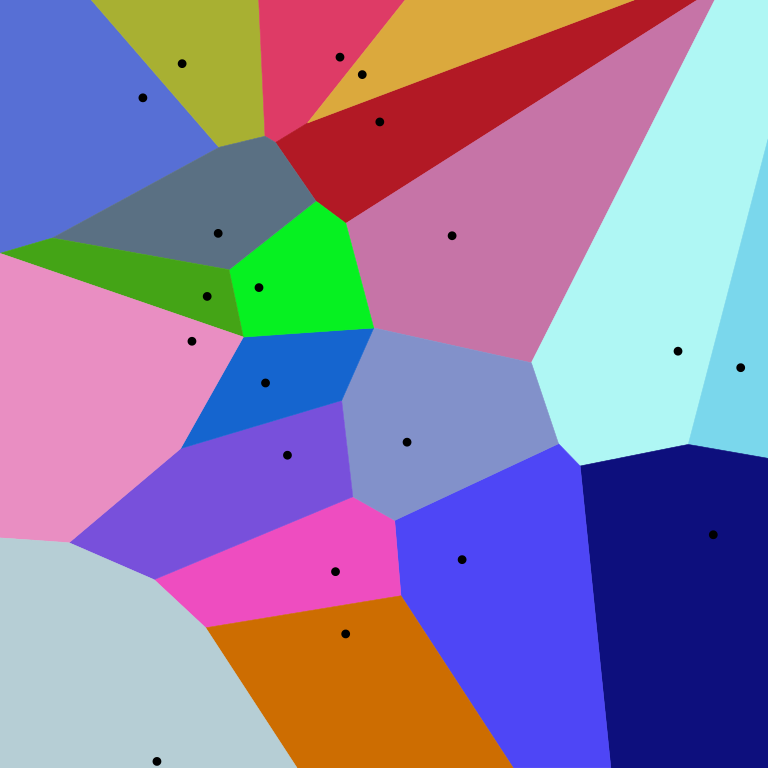
\includegraphics[width=0.7\textwidth]{euclidean_voronoi.png}}
    \only<2>{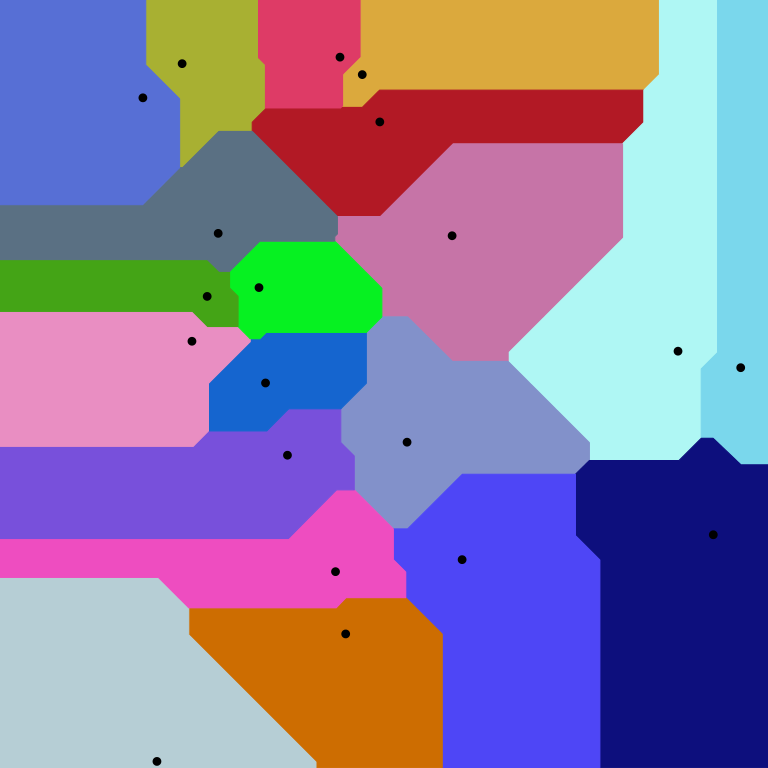
\includegraphics[width=0.7\textwidth]{manhattan_voronoi.png}}
  \end{center}
\end{frame}

\begin{frame}
  \frametitle{Some properties}
  \begin{itemize}[<+->]
  \item Any distance function can be used, giving a different diagram for the same set of points
    \vspace{\baselineskip}
  \item Using Euclidean distance, each cell is a convex polygon
    \vspace{\baselineskip}
  \item Using Euclidean distance, forms the dual of the Delaunay triangulation (more on this later)
    \vspace{\baselineskip}
  \item In general, a Voronoi diagram is relatively stable
  \end{itemize}
\end{frame}

\begin{frame}
  \frametitle{A simple algorithm: plane cutting}
  \begin{center}
    \only<1>{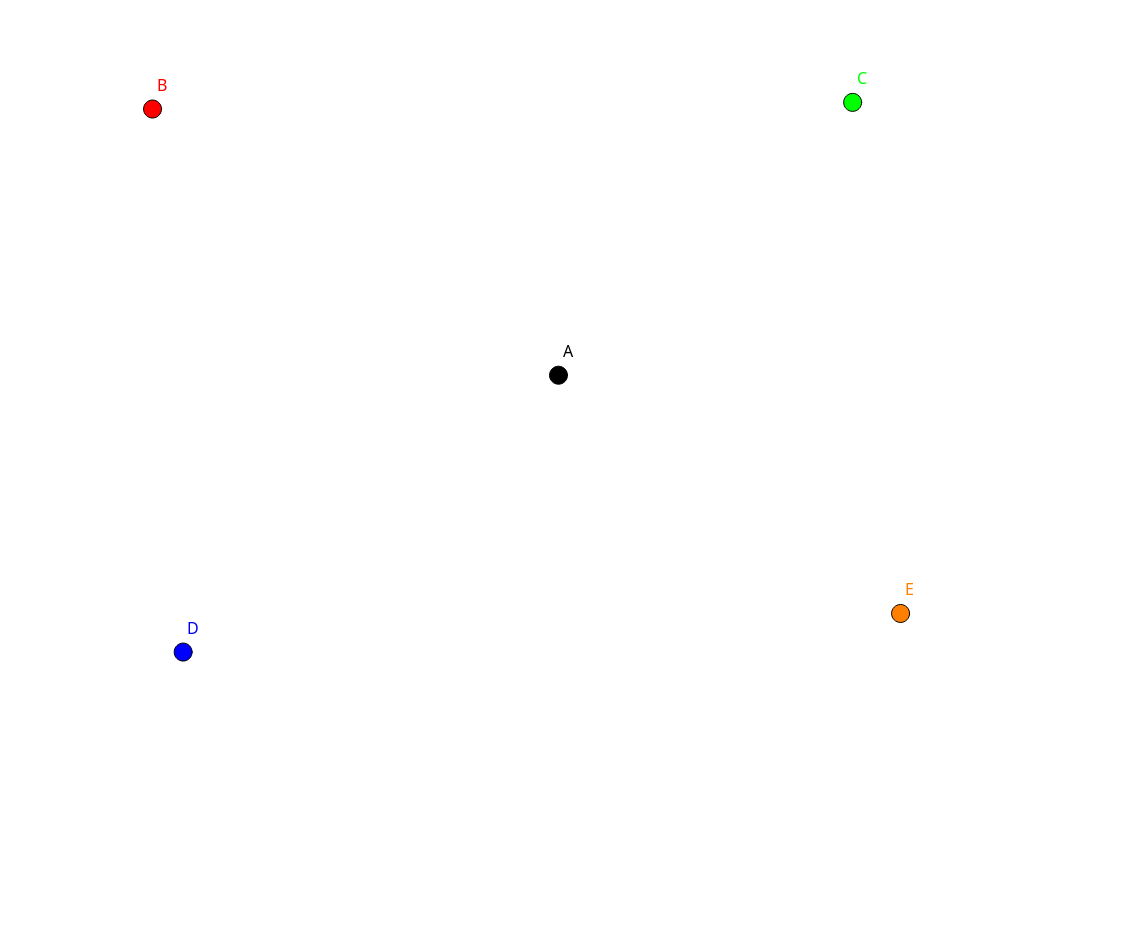
\includegraphics[width=\textwidth]{plane_cut_0.png}}
    \only<2>{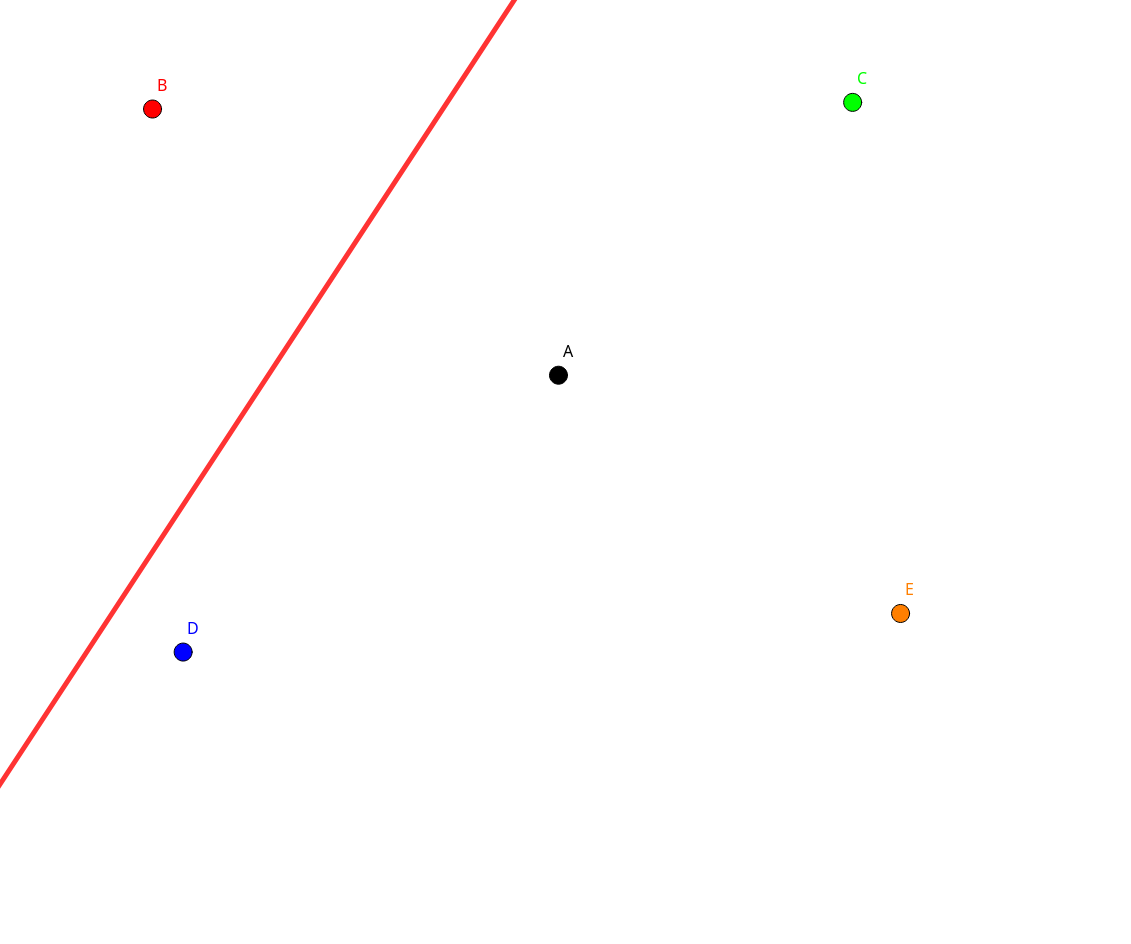
\includegraphics[width=\textwidth]{plane_cut_1.png}}
    \only<3>{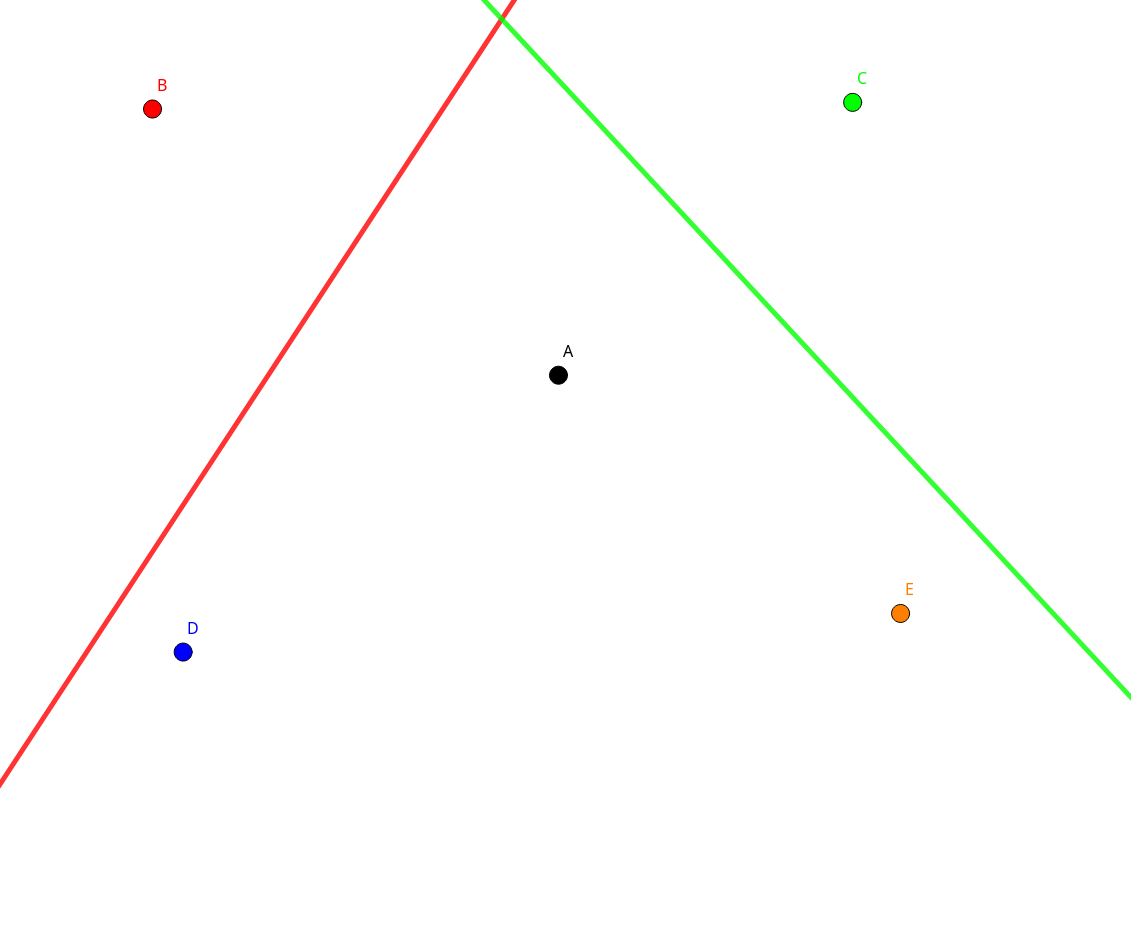
\includegraphics[width=\textwidth]{plane_cut_2.png}}
    \only<4>{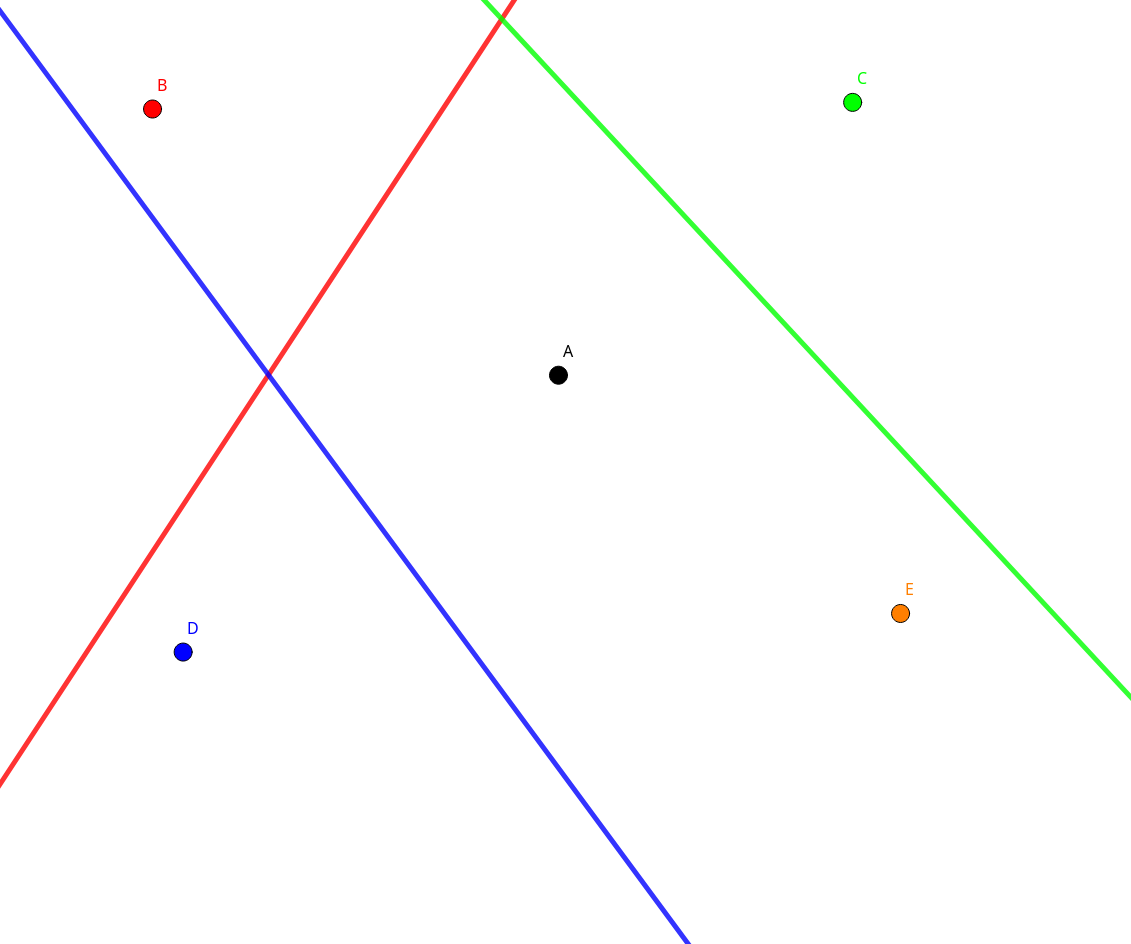
\includegraphics[width=\textwidth]{plane_cut_3.png}}
    \only<5>{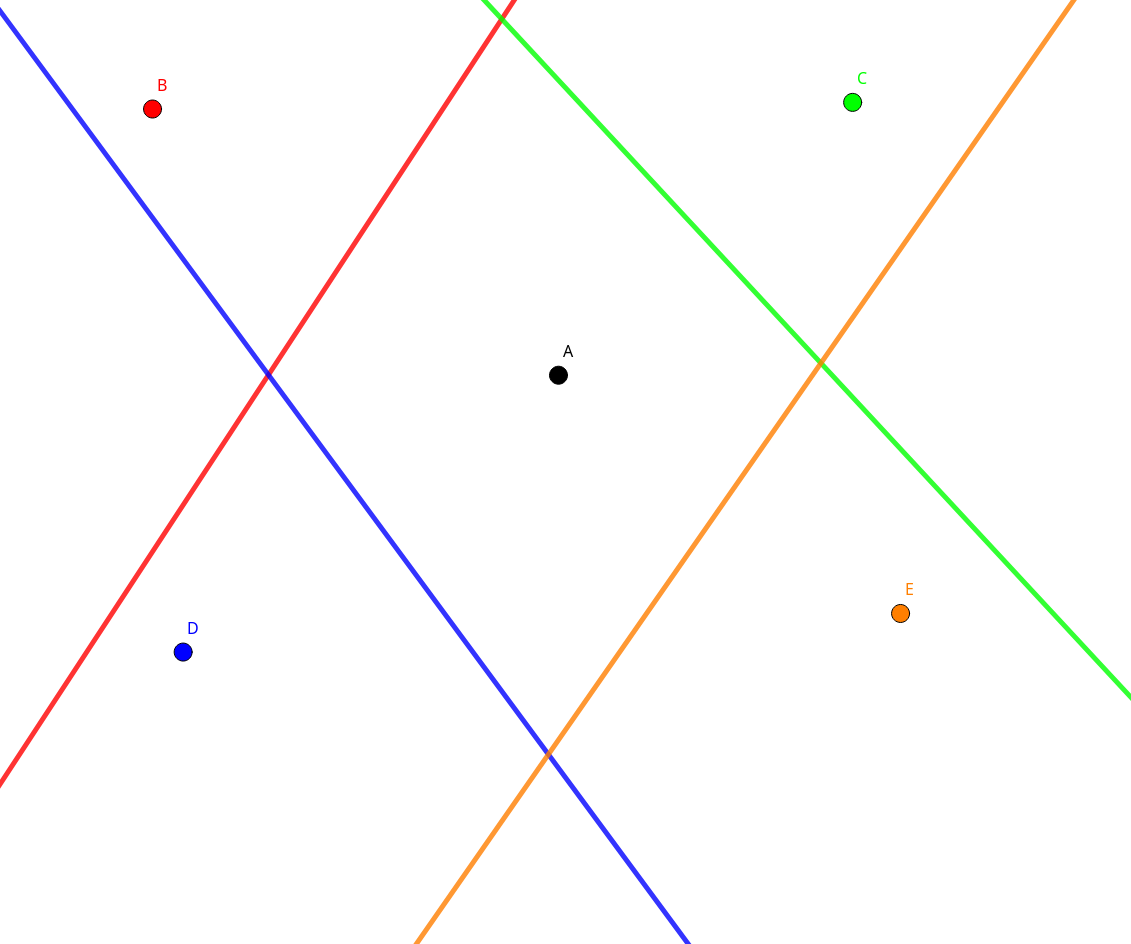
\includegraphics[width=\textwidth]{plane_cut_4.png}}
    \only<6>{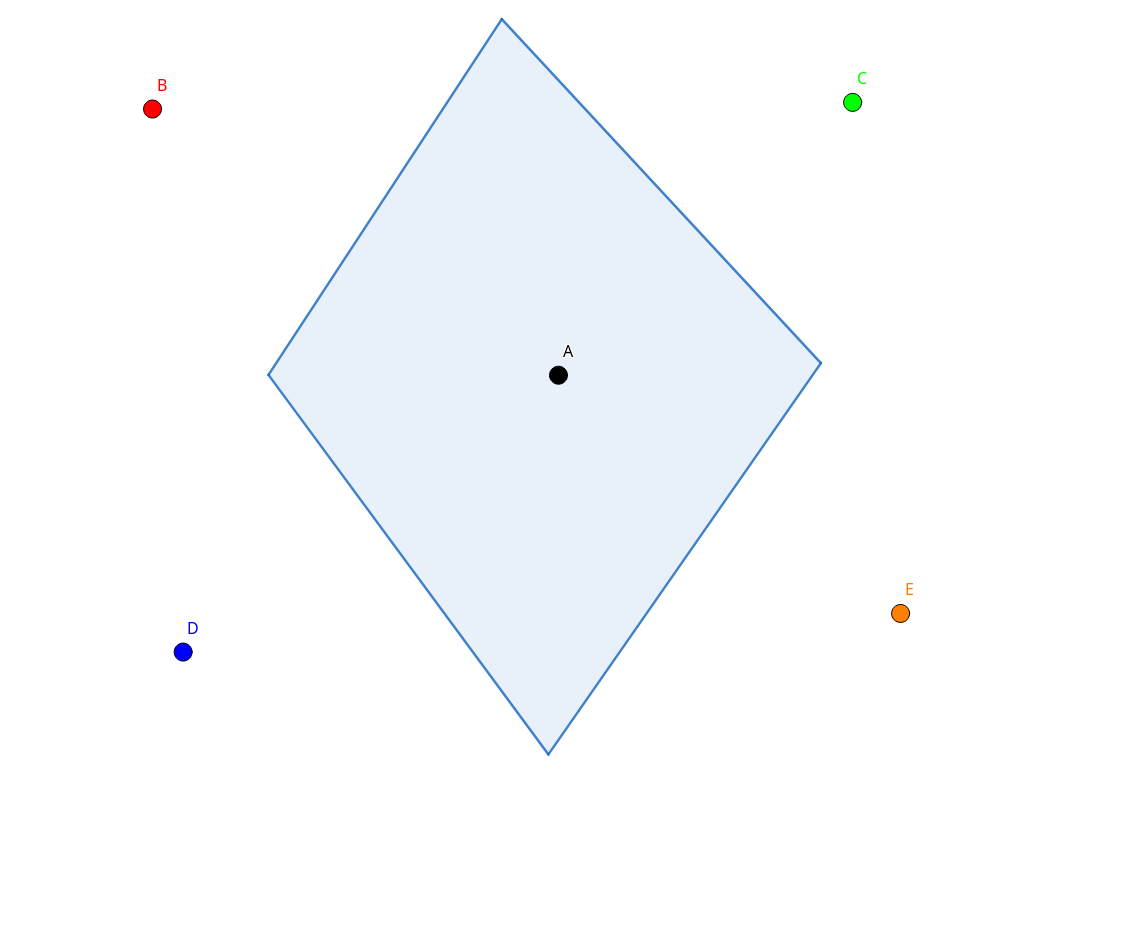
\includegraphics[width=\textwidth]{plane_cut_5.png}}
  \end{center}
\end{frame}

\begin{frame}
  \frametitle{Making the algorithm faster}
  \begin{itemize}[<+->]
  \item A single plane cut can be very expensive
    \vspace{\baselineskip}
  \item Can we skip a plane cut under certain conditions?
    \vspace{\baselineskip}
  \item Is there a preferred sequence of points to try?
  \end{itemize}
\end{frame}

\begin{frame}
  \frametitle{How to keep track of the distance between points}
  \begin{itemize}[<+->]
  \item Computing the distance between every pair of points is not ideal
    \vspace{\baselineskip}
  \item Is there a way to narrow the search down?
    \vspace{\baselineskip}
  \item Store the points in a way that associates ``close'' points
    \vspace{\baselineskip}
  \item Space partitioning data structures!
  \end{itemize}
\end{frame}

\begin{frame}
  \frametitle{Cell array}
  \begin{center}
    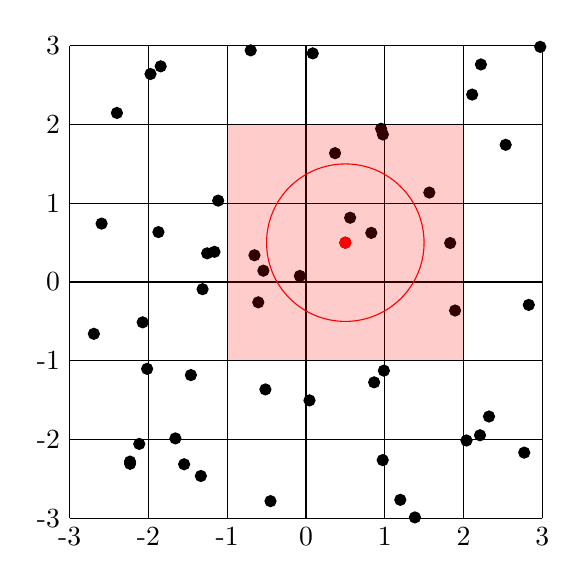
\begin{tikzpicture}
      \foreach \x in {-3,...,3}
      \draw (\x, -3) node[below] {\x} -- (\x, 3);
      \foreach \y in {-3,...,3}
      \draw (-3, \y) node[left] {\y} -- (3, \y);
      \foreach \x/\y in {-1.87338/0.634071, 0.976916/1.87369, 0.989637/-1.12538, -1.84498/2.73959, -1.65802/-1.98579, 2.82994/-0.290423, 1.56701/1.13608, 2.11091/2.3804, 2.97563/2.9869, -1.31302/-0.0908559, 1.89373/-0.36177, -2.23468/-2.28053, -0.540643/0.144004, -1.16172/0.383772, -2.23352/-2.30827, -0.654037/0.340101, -0.605618/-0.257674, -2.40062/2.14741, 0.829974/0.624413, 0.974933/-2.26176, 1.8317/0.495317, -1.54704/-2.31438, -1.97427/2.64208, -1.11494/1.03381, 1.38377/-2.9893, 0.561086/0.816618, -0.701837/2.9422, 2.5363/1.74276, 0.369634/1.63649, -0.450202/-2.78281, 2.32441/-1.70798, -1.46115/-1.18176, -2.07371/-0.511644, 0.865972/-1.27405, -0.0776774/0.0772877, -0.515025/-1.36365, -1.33475/-2.46312, -2.01722/-1.1023, -1.25491/0.36423, 2.77207/-2.16655, 1.19814/-2.76602, 2.21042/-1.94599, 0.954156/1.94636, -2.5953/0.741927, -2.69341/-0.657696, 2.03858/-2.01266, 2.22188/2.76312, -2.11703/-2.05583, 0.0448499/-1.50284, 0.0862097/2.90405}
      \filldraw (\x, \y) circle (2pt);
      \filldraw (0.5, 0.5) circle (2pt);
      \pause
      \filldraw[fill=red, draw=red] (0.5, 0.5) circle (2pt);
      \draw[draw=red] (0.5, 0.5) circle [radius=1];
      \pause
      \draw[fill=red, fill opacity=0.2] (-1, -1) -- (-1, 2) -- (2, 2) -- (2, -1) -- (-1, -1);
    \end{tikzpicture}
  \end{center}
\end{frame}

\begin{frame}
  \frametitle{K-D tree}
  \only<1>{Points: $(2,3)$, $(5,4)$, $(9,6)$, $(4,7)$, $(8,1)$, $(7,2)$}
  \only<2>{Points: $(2,3)$, $(5,4)$, $(9,6)$, $(4,7)$, $(8,1)$}
  \only<3>{Points: $(2,3)$, $(9,6)$, $(4,7)$, $(8,1)$}
  \only<4>{Points: $(2,3)$, $(4,7)$, $(8,1)$}
  \only<5>{Points: $(4,7)$, $(8,1)$}
  \only<6>{Points: $(8,1)$}
  \only<7>{All points added}
  \begin{columns}
    \begin{column}{0.7\textwidth}
      \begin{center}
        \begin{tikzpicture}[scale=0.6]
          \draw (0, 0) -- (0, 10) -- (10, 10) -- (10, 0) -- (0, 0);
          \foreach \x in {0,2,4,6,8,10}
          \draw (\x, 0) node[below] {\x};
          \foreach \y in {0,2,4,6,8,10}
          \draw (0, \y) node[left] {\y};
          \onslide<2->{\draw[color=red] (7, 0) -- (7, 10);}
          \onslide<2->{\filldraw (7, 2) circle (4pt);}
          \onslide<3->{\draw[color=blue] (0, 4) -- (7, 4);}
          \onslide<3->{\filldraw (5, 4) circle (4pt);}
          \onslide<4->{\draw[color=blue] (7, 6) -- (10, 6);}
          \onslide<4->{\filldraw (9, 6) circle (4pt);}
          \onslide<5->{\draw[color=red] (2, 0) -- (2, 4);}
          \onslide<5->{\filldraw (2, 3) circle (4pt);}
          \onslide<6->{\draw[color=red] (4, 4) -- (4, 10);}
          \onslide<6->{\filldraw (4, 7) circle (4pt);}
          \onslide<7->{\draw[color=red] (8, 0) -- (8, 6);}
          \onslide<7->{\filldraw (8, 1) circle (4pt);}
        \end{tikzpicture}
      \end{center}
    \end{column}
    \begin{column}{0.3\textwidth}
      \begin{center}
        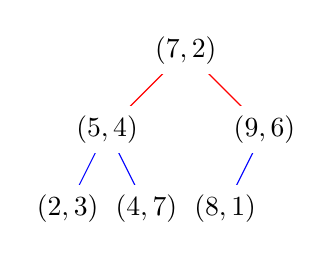
\begin{tikzpicture}
          \onslide<3->{\draw[color=red] (0, 0) -- (-1, -1);}
          \onslide<4->{\draw[color=red] (0, 0) -- (1, -1);}
          \onslide<5->{\draw[color=blue] (-1, -1) -- (-1.5, -2);}
          \onslide<6->{\draw[color=blue] (-1, -1) -- (-0.5, -2);}
          \onslide<7->{\draw[color=blue] (1, -1) -- (0.5, -2);}
          \onslide<2->{\draw (0, 0) node[fill=white] {$(7,2)$};}
          \onslide<3->{\draw (-1, -1) node[fill=white] {$(5,4)$};}
          \onslide<4->{\draw (1, -1) node[fill=white] {$(9,6)$};}
          \onslide<5->{\draw (-1.5, -2) node[fill=white] {$(2,3)$};}
          \onslide<6->{\draw (-0.5, -2) node[fill=white] {$(4,7)$};}
          \onslide<7->{\draw (0.5, -2) node[fill=white] {$(8,1)$};}
        \end{tikzpicture}
      \end{center}
    \end{column}
  \end{columns}
\end{frame}

\begin{frame}
  \frametitle{Tradeoffs between data structures}
  Cell array
  \begin{itemize}[<+->]
  \item Very good if points are uniformly distributed
  \item Can be tuned for different bucket size
  \item No guarantees for time to find the nearest point
  \item Works in any number of dimensions
  \item Add points at any time, constant time
  \end{itemize}
  \vspace{\baselineskip}
  \onslide<+->{K-D tree}
  \begin{itemize}[<+->]
  \item Handles uneven point distributions
  \item Find the nearest point in $O(\log n)$ time (average)
  \item Works in any number of dimensions (but at a cost)
  \item Adding points may require rebalancing $O(\log n)$
  \end{itemize}
\end{frame}

\begin{frame}
  \frametitle{Some applications}
  \begin{itemize}[<+->]
  \item Biology: skin pigment
    \vspace{\baselineskip}
  \item Image processing: can be used for image smoothing
    \vspace{\baselineskip}
  \item Fluid dynamics: generate finite regions for computational methods
    \vspace{\baselineskip}
  \item Robot navigation: follow edges to avoid obstacles
    \vspace{\baselineskip}
  \item Planning/mapping: identify the nearest location of interest
  \end{itemize}
\end{frame}

\begin{frame}
  \frametitle{Delaunay triangulation}
  \begin{center}
    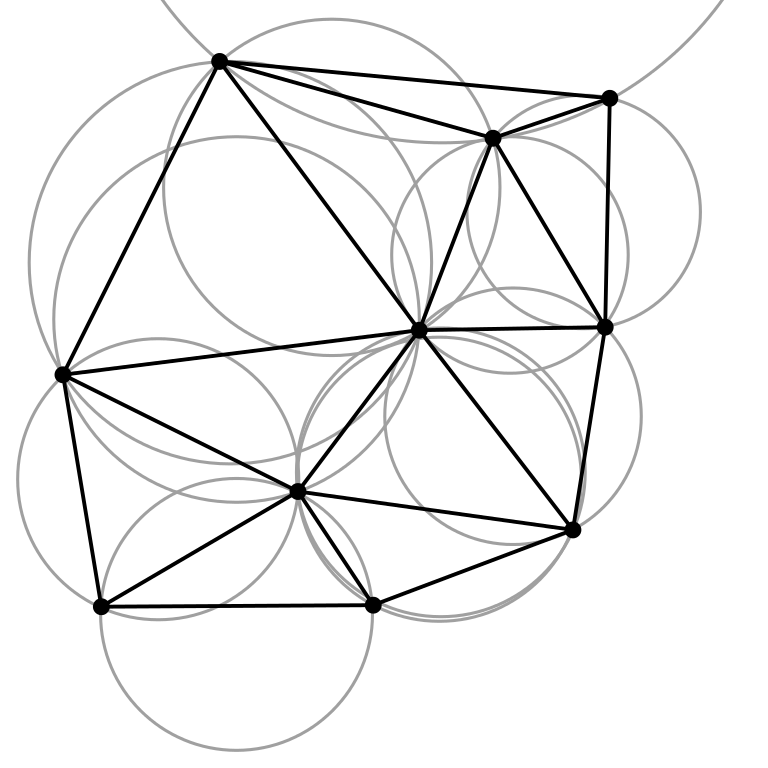
\includegraphics[width=0.8\textheight]{delaunay_simple.png}
  \end{center}
\end{frame}

\begin{frame}
  \frametitle{Delaunay triangulation for Voronoi tessellation}
  \begin{center}
    \only<1>{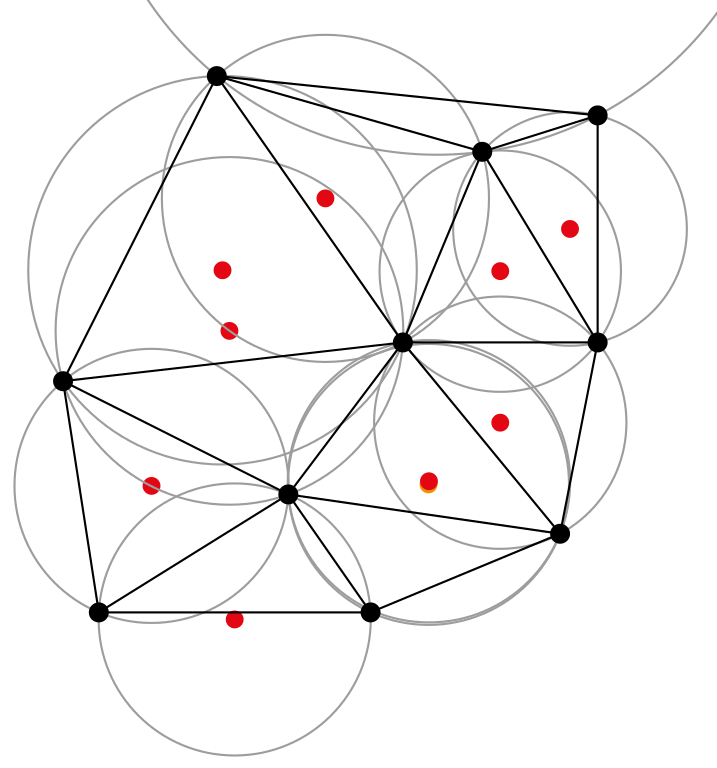
\includegraphics[width=0.8\textheight]{delaunay.png}}
    \only<2>{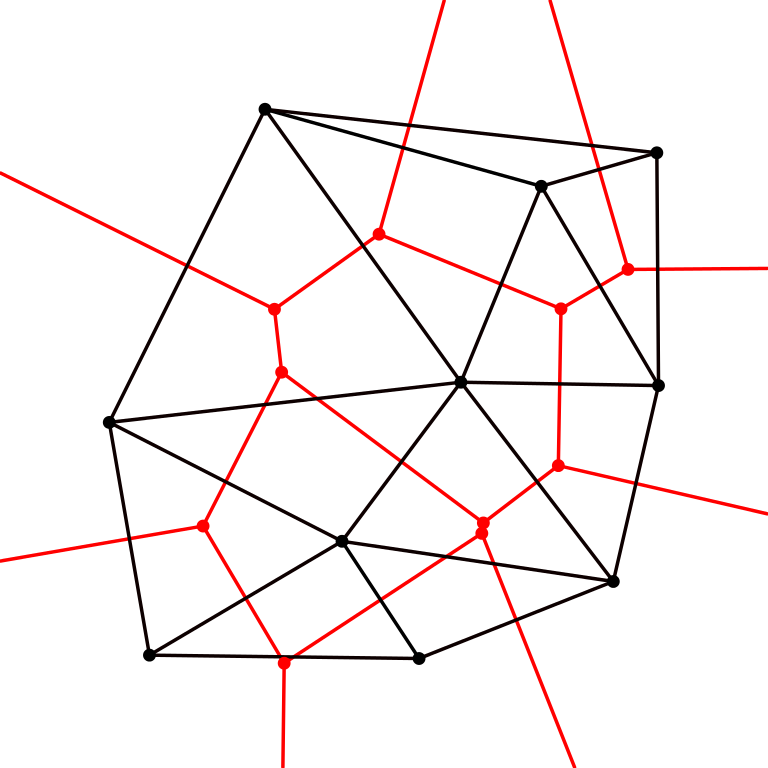
\includegraphics[width=0.8\textheight]{delaunay_voronoi.png}}
  \end{center}
\end{frame}

\begin{frame}
  \frametitle{Convex hull}
  \begin{center}
    \begin{tikzpicture}
      \filldraw (3,1) circle (2pt);
      \filldraw (-0.5,-2) circle (2pt);
      \filldraw (-1,2) circle (2pt);
      \filldraw (2,-1) circle (2pt);
      \filldraw (-3,-1) circle (2pt);
      \filldraw (0.5,0.5) circle (2pt);
      \filldraw (1,2) circle (2pt);
      \only<2>{\draw[color=red] (0,0) circle[radius=3.7];}
      \only<3>{\draw[color=red] (-3,-1) -- (-1,2) -- (1,2) -- (3,1) -- (2,-1) -- (-0.5,-2) -- (-3,-1);}
    \end{tikzpicture}
  \end{center}
\end{frame}

\begin{frame}
  \frametitle{Questions}
\end{frame}

\end{document}
